\documentclass{article}

\usepackage{polski}
\usepackage[UTF8]{inputenc}
\usepackage{graphicx}
\usepackage{float}
\usepackage[margin=1in]{geometry}
\usepackage{graphicx}
\usepackage{amsmath}
\usepackage{mathtools}
\usepackage{amssymb}
\usepackage{multirow}
\usepackage{changepage}
\usepackage{pbox}

\title{Sprawozdanie}
\begin{document}
	
\begin{center}
	\bgroup
	\def\arraystretch{1.5}
	\begin{tabular}{|c|c|c|c|c|c|}
		\hline
		EAIiIB & \multicolumn{2}{|c|}{\begin{tabular}{@{}c@{}} Autor 1\\ Autor 2\end{tabular}} & Rok II & Grupa 5 & Zespół 6 \\
		\hline
		\multicolumn{3}{|c|}{\begin{tabular}{c}Temat: \\ Współczynnik załamania ciał stałych \end{tabular}} & 
		\multicolumn{3}{|c|}{\begin{tabular}{c}Numer ćwiczenia: \\ 51 \end{tabular}} \\
		\hline
		Data wykonania & Data oddania & Zwrot do poprawki & Data oddania & Data zaliczenia & Ocena \\[8ex]
		\hline
	\end{tabular}
	\egroup
\end{center}  

	%WSTEP
\section{Cel ćwiczenia}
Wyznaczenie współczynnika załamania światła dla ciał stałych metodą mikroskopu. 
Zbadanie zależności współczynnika załamania od długości fali.
\section{Wstęp teoretyczny}
Gdy wiązka światła przechodzi przez dwa ośrodki o różnych własnościach optycznych, to na powierzchni granicznej częściowo zostaje odbita, częściowo zaś przechodzi do drugiego środowiska, ulegając załamaniu.
Prawo załamania:
$$\frac{sin \alpha}{sin \beta} = n$$ 
Wielkość n jest stała zwaną współczynnikiem załamania ośrodka 2 względem ośrodka 1. 
Współczynnik załamania zależy od długości fali światła padającego. 


\begin{figure}[!htb]
	\centering
	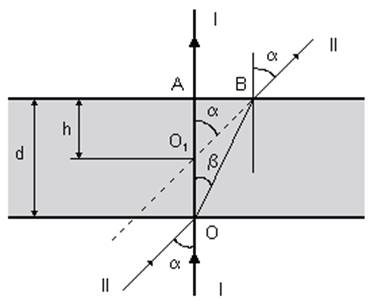
\includegraphics[width=90mm]{image006.jpg}
	\caption{Powstanie  pozornego  obrazu  $O_{1}$ punktu  $O$  leżącego  na  dolnej  powierzchni płytki płaskorównoległej }
\end{figure}
\clearpage
\section{Układ pomiarowy}
W skład układu pomiarowego wchodzą: 
\begin{enumerate}
\item Mikroskop wyposażony w czujnik mikrometryczny i nasadkę krzyżową
\item Śruba mikrometryczna. 
\item Zestaw płytek szklanych i z pleksiglasu, różnej grubości
\end{enumerate}
\section{Wyniki pomiarów}

	\begin{adjustwidth}{-1cm}{}
\def\arraystretch{1.3}
\begin{center}
	\begin{tabular}{|c|c|c|c|c|}
		\hline
		\multicolumn{5}{|l|}{\begin{tabular}{l} Materiał: pleksiglas\\ Grubość rzeczywista: $d$ =4,75 [mm]\\ niepewność $u(d)$=0,01 [mm] \end{tabular}}\\
		\hline
		\multirow{3}{*}{Lp.} & \multicolumn{2}{|c|}{Wskazanie czujnika} & \begin{tabular}{c}Grubość \\pozorna\end{tabular} &\begin{tabular}{c}Współczynnik \\załamania\end{tabular} \\ \cline{2-5}
		& \parbox[c]{1.8 cm}{\centering $a_{d}$}  & $a_{g}$ & $h=a_{d}-a_{g}$ & \multirow{2}{*}{$n=\frac{d}{h}$}\\ \cline{2-4}
		& [mm] & [mm] & [mm] & \\ 
		
		\hline
		1. & 8,43 & 5,22& 3,21& 1,480\\
		\hline
		2. & 8,47 & 5,25& 3,22& 1,475\\
		\hline
		3. & 8,40 & 5,25& 3,15& 1,508\\
		\hline
		4. & 8,43 & 5,28& 3,15& 1,507\\
		\hline
		5. & 8,46 & 5,31& 3,15& 1,508\\
		\hline
		6. & 8,44 & 5,26& 3,18& 1,494\\
		\hline
		7. & 8,46 & 5,22& 3,24& 1,466\\
		\hline
		8. & 8,46 & 5,31& 3,15& 1,506\\
		\hline
		9. & 8,46 & 5,22& 3,24& 1,466\\
		\hline
		10.& 8,43 & 5,29& 3,14& 1,513\\
		\hline
		\multicolumn{2}{c|}{}&\begin{tabular}{c}Wartość \\ średnia \end{tabular}&3,18 &1,492 \\
		\cline{3-5}
		\multicolumn{2}{c|}{}&\begin{tabular}{c}Niepewność \end{tabular}& 0,0379& 0,01804\\
		\cline{3-5}
	\end{tabular}
	\end{center}
\end{adjustwidth}




\begin{adjustwidth}{-1cm}{}
	\def\arraystretch{1.3}
	\begin{center}
	\begin{tabular}{|c|c|c|c|c|c|c|}
		\hline
		\multicolumn{4}{|l|}{Materiał: pleksiglas} & \multicolumn{3}{|l|}{Grubość rzeczywista $d$=4,75[mm]}\\
		\hline
		\multicolumn{2}{|c|}{\parbox[c]{2.4cm}{\centering Długość fali}} & \multicolumn{2}{|c|}{Wskazanie czujnika} & \begin{tabular}{c}Grubość \\pozorna\end{tabular} &\begin{tabular}{@{}c@{}}Współczynnik \\załamania\end{tabular} & \begin{tabular}{c}Wartość \\średnia\end{tabular} \\ 
		\hline
		\multicolumn{2}{|c|}{$\lambda$} & \parbox[c]{1.4cm}{\centering $a_{d}$}  & $a_{g}$ & $h=a_{d}-a_{g}$ & \multirow{2}{*}{$n=\frac{d}{h}$} & \multirow{2}{*}{$n_{sr}$} \\ 
		\cline{1-5}
		\multicolumn{2}{|c|}{[$\mu m$]} & [mm] &[mm] &[mm] & & \\ 
		\hline
				\multirow{5}{*}{I} & \multirow{5}{*}{\parbox[c]{1cm}{Niebieski 0,48}} & 8,40& 5,25& 3,15& 1,508& \multirow{5}{*}{1,503} \\
				\cline{3-6}
				& & 8,42& 5,25& 3,17& 1,498& \\
				\cline{3-6}
				& & 8,43& 5,29& 3,14& 1,515& \\
				\cline{3-6}
				& & 8,44& 5,27& 3,17& 1,500& \\
				\cline{3-6}
				& & 8,41& 5,23& 3,18& 1,493& \\
				\hline
				\multirow{5}{*}{II} & \multirow{5}{*}{\parbox[c]{1cm}{Zielony 0,50}} & 8,36& 5,33& 3,03& 1,568& \multirow{5}{*}{1,503} \\
				\cline{3-6}
				& & 8,43& 5,26& 3,17& 1,498& \\
				\cline{3-6}
				& & 8,44& 5,24& 3,20& 1,484& \\
				\cline{3-6}
				& & 8,44& 5,23& 3,21& 1,480& \\
				\cline{3-6}
				& & 8,46& 5,26& 3,20& 1,484& \\
				\hline
				\multirow{5}{*}{III} & \multirow{5}{*}{\parbox[c]{1cm}{Żółty 0,59}} & 8,45& 5,27& 3,18& 1,494& \multirow{5}{*}{1,488} \\
				\cline{3-6}
				& & 8,42& 5,21& 3,21& 1,477& \\
				\cline{3-6}
				& & 8,45& 5,24& 3,21& 1,480& \\
				\cline{3-6}
				& & 8,44& 5,25& 3,19& 1,489& \\
				\cline{3-6}
				& & 8,44& 5,27& 3,17& 1,498& \\
				\hline
		\multirow{5}{*}{IV} & \multirow{5}{*}{\parbox[c]{1cm}{Czerwony 0,63}} & 8,39& 5,23& 3,16& 1,503& \multirow{5}{*}{1,507}\\
		\cline{3-6}
		& & 8,42& 5,27& 3,15& 1,508& \\
		\cline{3-6}
		& & 8,42& 5,27& 3,15& 1,508& \\
		\cline{3-6}
		& & 8,41& 5,26& 3,15& 1,508& \\
		\cline{3-6}
		& & 8,42& 5,27& 3,15& 1,508& \\
		\hline

	\end{tabular}
\end{center}
\end{adjustwidth}
	
\section{Obliczenia}
\begin{enumerate}
	\item Obliczamy wartość współczynnika załamania światła korzystając ze wzoru $n=\frac{d}{h}$
	\item Niepewność grubości płytki rzeczywistej przyjmujemy $u(d) = 0,01$ [mm]
	\item Niepewność grubości pozornej $u(h)$ dla poszczególnych rodzajów światła.
	\begin{adjustwidth}{-1cm}{}
\def\arraystretch{1.3}
\begin{center}
	\begin{tabular}{|c|c|c|}
		\hline
		\multicolumn{1}{|c|}{\begin{tabular}{@{}c@{}}Rodzaj \\światła\end{tabular}}& \begin{tabular}{@{}c@{}}Grubość \\pozorna $h$[mm]\end{tabular} & Niepewność $u(h)$ [mm] \\
		\hline
		Niebieskie & 3,16 & 0,0165 \\
		\hline
		Zielone& 3,16 & 0,0673 \\
		\hline
		Białe & 3,18 & 0,0379 \\
		\hline
		Żółte& 3,19 & 0,0172 \\
		\hline
		Czerwone& 3,15 & 0,0040 \\
		\hline 
	\end{tabular}
	\end{center}
\end{adjustwidth}

	\item Wyznaczamy niepewność obliczonego współczynnika załamania światła.\\
	Niepewność współczynnika załamania światła:
$$ u(n) =\sqrt{\bigg(\frac{\partial n}{\partial d}u(d)\bigg)^2+\bigg(\frac{\partial n}{\partial h}u(h)\bigg)^2} = \sqrt{\bigg(\frac{1}{h}u(d)\bigg)^2+\bigg(\frac{-d}{h^2}u(h)\bigg)^2}$$

	\item Zestawienie wyników
	\begin{adjustwidth}{-1cm}{}
\def\arraystretch{1.3}
\begin{center}
	\begin{tabular}{|c|c|c|c|}
		\hline
		\multicolumn{1}{|c|}{\begin{tabular}{@{}c@{}}Rodzaj \\światła\end{tabular}}& \begin{tabular}{@{}c@{}}Współczynnik \\załamania $n$ \end{tabular} & Niepewność $u(n)$& \begin{tabular}{@{}c@{}}Zgodność z wartością tablicową \\w granicach \\niepewności rozszerzonej\end{tabular}\\
		\hline
		Niebieskie& 1,503 & 0,00847 & TAK\\
		\hline
		Zielone & 1,503 & 0,03215 & TAK\\
		\hline 		
		Białe &1,492 & 0,01804 & TAK \\
		\hline
		Żółte & 1,488 & 0,00860 & TAK\\
		\hline
		Czerwone & 1,507 & 0,00370 & NIE\\
		\hline
	\end{tabular}
	\end{center}
\end{adjustwidth}
\end{enumerate}



\section{Wnioski}
Otrzymana wartość współczynnika załamania po oświetleniu płytki z pleksiglasu światłem białym jest zgodna z wartością tablicową (1,5) w granicach niepewności.
Po oświetleniu płytki z pleksiglasu światłem o różnej długości możemy stwierdzić, że współczynnik załamania zależy od długość fali (zjawisko dyspersji). Wyznaczony współczynnik załamania po oświetleniu światłem barwy czerwonej nie odpowiada oczekiwanemu wynikowi. Prawdopodobnie przyczyną takiego wyniku jest mała dokładność metody pomiaru, ponieważ stwierdzenie czy obraz na wyświetlaczu mikroskopu jest już wystarczająco ostry jest bardzo subiektywne.
\end{document}